\documentclass[a4paper,11pt]{article}
%%%%%%%%%%%%%%%%%%%%%%%%%%%%%%%%%%%%%%%%%%%%%%%%%%%%%%%%%%%%%%%%%%%%%%%%%%%%%%%%%%%%%%%%%%%%%%%%%%%%%%%%%%%%%%%%%%%%%%%%%%%%
\usepackage[T1]{fontenc}
\usepackage[utf8]{inputenc}
\usepackage{graphicx}
\usepackage{pdfpages} 
\usepackage{amsmath}
 \usepackage{amssymb}
\usepackage{natbib}
\usepackage[dvips]{color}
\usepackage{subfigure}
\usepackage{verbatim}
\usepackage{hyperref}

\bibpunct{(}{)}{;}{a}{,}{,}

\textheight 24cm \textwidth 17cm \topmargin-2cm
%% \evensidemargin   -0.25cm
\oddsidemargin-0.2cm
%\pagestyle{empty}
\renewcommand{\baselinestretch}{1}

\begin{document}

\title{A study to Deploy \\ Wikipedia NER (Named Entity Recognition) \\as scalable service in real time}


\author{{Roberto Maestre \footnote{rmaestre@paradigmatecnologico.com}  
				Angel Cortes \footnote{acortes@paradigmatecnologico.com} 
				Alejandro Gonzalez \footnote{agonzalez@paradigmatecnologico.com} 
				Ruben Abad \footnote{rabad@paradigmatecnologico.com}
				} \\
{\small Paradigma Labs \\ Paradigma Tecnológico \\ 2012}}

\date{}
\maketitle

%\title{}

%\address{}


\begin{abstract} This document shows the main behavior of Wikipedia NER service in order to provides a few basic steps to load the library and run the service in a production environment. Also a theoretical study based on Continuous-Time Markov Chains is provided to find main parameters to design a stable production environment. A simulation is performed in order to find the optimus parameters to our system and test it.
\end{abstract}


\ \\
KEY WORDS: Named Entity Recognition, Classification, Graphs, Continuous-Time Markov chains.




\section{Introduction and main NER concepts}
NER is one of the classic problem in the AI/semantic field. Paradigma Labs provides a service (supported by Tornado) to perform this operation. Based on Wikipedia categories and articles, we can provide a 25.000.000 million of success lookups. 
\\
\\
Based on Wikipedia dumps\footnote{\url{http://dumps.wikimedia.org/enwiki/}}\footnote{\url{http://www.mediawiki.org/wiki/Manual:Database\_layout}} and using hadoop systems\footnote{\url{http://hadoop.apache.org/}} in order to handle this huge information, we can create our semantic network based on two pairs: categories and articles (in the semantic network, articles are called concepts), following the next definition:
\begin{equation}
\begin{array}{l}
\displaystyle A = \{a_1 , ... , a_n\} \\
\displaystyle B = \{b_1 , ... , b_k\} \\
\displaystyle a_x = b_y \Leftrightarrow x = y \\
\displaystyle a \in V, \displaystyle b \in V
\\
\displaystyle G=(V , E) \\
\displaystyle V = \emptyset \\
\displaystyle E \subseteq \{(c,d) \in V\times V : c \neq d \} \\
\end{array}
\end{equation}
where $A$ is the set of categories, $B$ is the set of articles in Wikipedia and $G$ the semantic network.
\\
\\
Wikipedia provides constant updates, each month is released a complete $DUMP$ with Wikipedia structure, several categories and articles are added and other are removed. Our NER is changing across the time.


\begin{figure}[htb]
\begin{center}
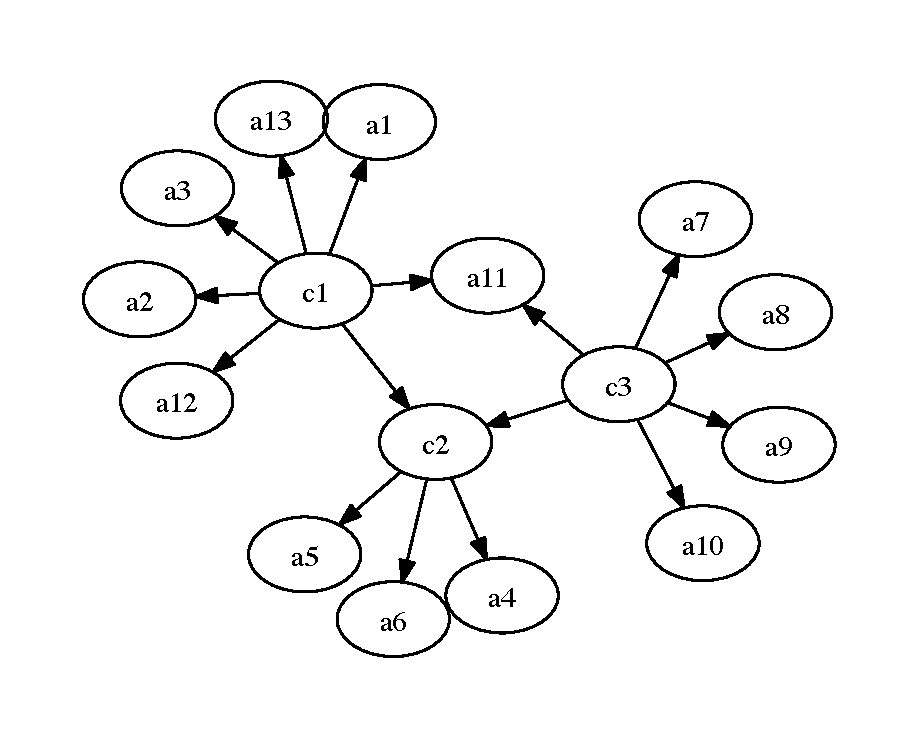
\includegraphics[width=0.5\textwidth]{img/wikipedia_structure.pdf}
\caption{Wikipedia semantic network}
\end{center}
\end{figure}
\\
\\
This service only provides Spanish-entities names, however, could be easily implemented other services for several languages\footnote{\url{http://meta.wikimedia.org/wiki/List\_of\_Wikipedias}}. The number of entities recognized could change directly related with the language implementation.
\\
This service, can support a real time operations against itself, for this reason, it is implemented using Gunicorn and Tornados services. Unicorn is able to create several Tornados services like threads (actually process). Finally, Monit\footnote{\url{http://linux.die.net/man/1/monit}} will track Gunicorn process.





\newpage
\section{NER as Tornado service}
Tornado is an open source version of the scalable, non-blocking web server and tools that power FriendFeed. The FriendFeed application is written using a web framework that looks a bit like web.py or Google's webapp, but with additional tools and optimizations to take advantage of the underlying non-blocking infrastructure. Because it is non-blocking and uses epoll\footnote{\url{http://www.kernel.org/doc/man-pages/online/pages/man4/epoll.4.html}} or kqueue, it can handle thousands of simultaneous standing connections, which means it is ideal for real-time web services.
\\
At FriendFeed, they use nginx\footnote{\url{http://nginx.org/}} as a load balancer and static file server, however, we are going to use Gunicorn to create a multiprocess server and finally we are going to use a nginx too to balance different servers.
\\

Once this service is up in debug mode, i.e.: {\bf > python server.py}, we can access by means of the next URI:
\begin{verbatim}
http://78.46.84.166:8000/?token=d41d8cd98f00&inlinks_threshold=1&
                       text=el%20banco%20de%20espa%C3%B1a%20va%20a%20quebrar
\end{verbatim}
and response will be:
\begin{verbatim}
{
text: "el banco de españa va a quebrar",
  results: {
    banco de españa: {
        start: 3,
        entity: false,
        end: 20,
        composition: false,
        inlinks: 341
    },
    quebrar: {
        start: 25,
        entity: false,
        end: 33,
        composition: false,
        inlinks: 1
    },
    el banco: {
        start: 1,
        entity: true,
        end: 9,
        composition: false,
        inlinks: 35
    }
  }  
}
\end{verbatim}
As we can see in the picture above, NER service detect several Entities like "banco de españa", "quebrar" and "el banco". This service is able to detect overlaps between concepts, like in "banco de españa" y "el banco". Each user has a unique token to consume this service.
\\
\\
Another important concept is the {\bf inlink} concept. Inlink concept means the number of article pointing to it; e.g.: "banco de españa" has a higher inlink than "el banco", it means that "banco de españa" is more important (as semantic sense) than "banco". We are able to calculate this parameter (and the whole structure) by means of PIG and hadoop process.
\\ We provide the pig script :
\\
\begin{verbatim}
A = LOAD 'hdfs://web40:54310/user/hadoop/input/en_id_page.tsv.gz' 
             USING PigStorage('\t') AS (page_id , page);
B = LOAD 'hdfs://web40:54310/user/hadoop/input/en_categories_links.tsv.gz' 
             USING PigStorage('\t') AS (page_id_to , page_from);

C = JOIN A by page_id, B by page_id_to;
LINKS = FOREACH C GENERATE $1,$3;
LINKS_TO = FOREACH LINKS GENERATE $1;
U_LINKS_TO = DISTINCT LINKS_TO;
CATEGORIES = JOIN LINKS by $0, U_LINKS_TO by $0;
U_CATEGORIES = FOREACH CATEGORIES GENERATE $0,$1;
H = cogroup LINKS by $0, U_CATEGORIES by $1;
I = filter H by COUNT(U_CATEGORIES) == 0;
PAGES_ID = FOREACH I GENERATE $0;
U_PAGES_ID = DISTINCT PAGES_ID;
PAGES = JOIN LINKS by $0,U_PAGES_ID by $0;
U_PAGES = FOREACH PAGES GENERATE $0,$1;

STORE U_CATEGORIES INTO 'hdfs://web40:54310/user/hadoop/categories/';
STORE U_PAGES INTO 'hdfs://web40:54310/user/hadoop/pages';
\end{verbatim}
\\
\\
Mandatory parameters for this service are:
\begin{itemize}
\item {\bf text} =  (A string) Into this text, NER extract all possible entities.
\item {\bf inlinks\_threshold} =  (An integer) Filter parameter to remove entities whit a lower threshold.
\item {\bf token} =  Token (like an id) to acces into the application.
\end{itemize}





\newpage
\section{Gunicorn as scalable service}
Gunicorn is based on the pre-fork worker model. This means that there is a central master process that manages a set of worker processes. The master never knows anything about individual clients. All requests and responses are handled completely by worker processes.
\\
There's also a Tornado worker class. It can be used to write applications using the Tornado framework. Although the Tornado workers are capable of serving a WSGI application, this is not a recommended configuration.
\\
\\
How Many Workers?
\\
Do not scale the number of workers to the number of clients you expect to have. Gunicorn should only need 4-12 worker processes to handle hundreds or thousands of requests per second.
\\
\\
Gunicorn relies on the operating system to provide all of the load balancing when handling requests. Generally we recommend (2 x \$num\_cores) + 1 as the number of workers to start off with. While not overly scientific, the formula is based on the assumption that for a given core, one worker will be reading or writing from the socket while the other worker is processing a request.
\\
\\
We should install several packages:
\begin{verbatim}
sudo easy_install multiprocessing
sudo easy_install tornado
sudo easy_install gunicorn
\end{verbatim}
\\
\\
We can execute our services trough the next command:
\begin{verbatim}
nohup gunicorn  --workers 4 
                --limit-request-line 4094 
                --limit-request-fields 4 
                --backlog 2000
                -b 0.0.0.0:8000 
                -k egg:gunicorn#tornado server:app &
\end{verbatim}
\\
\\
Tornado service skeleton could be:
\begin{verbatim}
# -*- coding: utf-8 -*-
import tornado.ioloop
from tornado.web import Application, RequestHandler, asynchronous
from tornado.ioloop import IOLoop

# Main class
class NerService(tornado.web.RequestHandler):
    def get(self):
    
    
# run application
app = tornado.web.Application([
    (r"/", NerService, dict(...parameters...),
    ])
    
# To test single server file"
app.listen(8000)
tornado.ioloop.IOLoop.instance().start()
\end{verbatim}




\newpage
\section{Monit}
Monit\footnote{\url{http://mmonit.com/monit/}} is a free open source utility for managing and monitoring, processes, programs, files, directories and filesystems on a UNIX system. Monit conducts automatic maintenance and repair and can execute meaningful causal actions in error situations.
\\
\\
Monit is able to:
\begin{itemize}
\item Start, stop, restart processes and services
\tiem Check system CPU, memory and load
\item Alert reports
\item Alert notification
\end{itemize}
\\
The next script can be used to manage gunicron like a service:
\begin{verbatim}
#!/bin/bash
 #MODIFY TO USE YOUR OWN SERVICE
export SERVICE_PATH="/home/desa/ner_service"
export SERVICE_PID="$SERVICE_PATH/gunicor_service.pid"
export SERVICE_LOG="$SERVICE_PATH/service.log"
export TIMEOUT=3
export GUNICORN_OPTS="--workers 4 --limit-request-line 4094 --limit-request-fields 4 -k egg:gunicorn#tornado server:app"
export GUNICORN_BIND="0.0.0.0:8000"

####DO NOT MODIFY#######
case $1 in
  start)
  if [ ! -z "$SERVICE_PID" ]; then
          if [ -f "$SERVICE_PID" ]; then
            pid=`cat "$SERVICE_PID"`
            running=`ps ax | grep "^[[:blank:]]*$pid[^0-9]" | wc -l`
            if [ $running != "0" ]; then
              echo "process already running. Start aborted!";
              exit 1
            else
              rm -f "$SERVICE_PID"
            fi
          fi
      fi
      cd $SERVICE_PATH
      #Run the gunicorn
      nohup gunicorn $GUNICORN_OPTS -b $GUNICORN_BIND --pid $SERVICE_PID >> $SERVICE_LOG &
  ;;
  stop)
  if [ ! -z "$SERVICE_PID" ]; then
          if [ -f "$SERVICE_PID" ]; then
            pid=`cat "$SERVICE_PID"`
            running=`ps ax | grep "^[[:blank:]]*$pid[^0-9]" | wc -l`
            if [ $running != "0" ]; then
              cd $SERVICE_PATH
              #Kill the gunicorn, he should stop all the childs
              kill -9 $pid
              #echo "DEBUG: Aqui ya habria mandado parar al servicio"
            else
              rm -f "$SERVICE_PID"
              echo "no process running for pid in file. Cleaning pid file";
              exit 0
            fi
          else
            echo "can not find the pid file. Already stopped?";
            exit 0
          fi
      fi
      #Validation to destroy gunicorn if still running "TIMEOUT" seconds after 
      #shutdown order
      echo "Waiting $TIMEOUT seconds for gunicorn shutdow all threads"
      sleep $TIMEOUT
      running=`ps ax | grep "^[[:blank:]]*$pid[^0-9]" | wc -l`
            if [ $running != "0" ]; then
              kill -9 $pid
              if [ -f "$SERVICE_PID" ]; then
                      rm -f "$SERVICE_PID"
                      echo "gunicorn with PID $pid stopped with SIGKILL. Cleaning pid file";
                      exit 0
              fi
            else
              echo "Stoped gratefully";
              exit 0
            fi
  ;;
  *)
  echo "Usage: start (start|stop)" ;;
  esac
\end{verbatim}


\newpage
\section{Continuous-Time Markov chains}
Through Markov chains\footnote{\url{http://lyrawww.uvt.nl/~blanc/qm-blanc.pdf}} we have the ideal framework to create simulations in order to estimate the load and stress of our service. Derivate from Continuous-Time Markov Chains, we have the Tail Theory\footnote{\url{http://en.wikipedia.org/wiki/M/M/c/k}}, which could apply directly to our problem and simplify the operations.
\\
Main parameters are:
\begin{itemize}
\item $\lambda$: Is related with incoming tax to our system
\item $\mu$: Is related with service time
\item $c$: Is the number of parallel services (in our case are tornados servers running in parallel with gunicorn)
\item $k$ is the maximum capacity of the tail
\end{itemize}
Now, we are able to model our system like a $M_1$/$M_2$/c/k, where:
\begin{itemize}
\item $M_1$ $\sim P(\lambda)$
\item $M_2$ $\sim Exp(\mu)$
\end{itemize}


\begin{figure}[htb]
\begin{center}
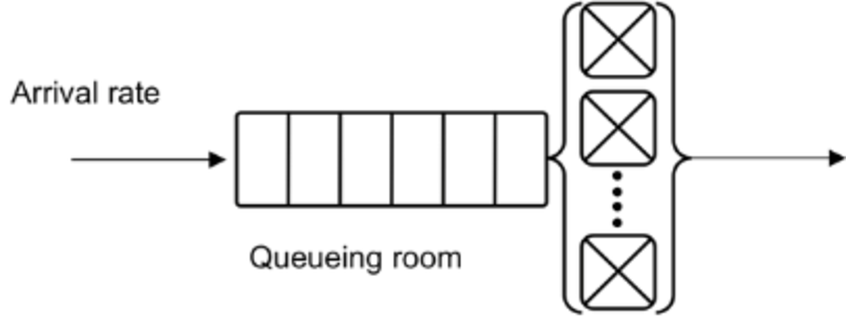
\includegraphics[width=0.6\textwidth]{img/tail.pdf}
\caption{Service like a tail with "c" servers and maximum capacity "k"}
\end{center}
\end{figure}
\\
We can derivate the next parameters
\begin{itemize}
\item $\rho$: Is related with the use intensity of the system $\displaystyle\frac{\lambda}{k\mu}$ and always must holds that $\rho < 1$ (stability condition).
\item We can define $\mu_n$ where $n$ is the number of clients at a given state.
\begin{equation*}
\mu_n = \left \{
\begin{matrix}
n\mu & 0 \leq n \leq c\\
c\mu & c \leq n \leq k\\
\end{matrix} \right.
\end{equation*}
\item Probability to find $n$ clients into the system is defined as:

\begin{equation*}
P_n = \left \{
\begin{matrix}
\displaystyle \frac{\lambda^n}{n! \mu^n} P_0 &  1 \leq n < c\\
\displaystyle \frac{\lambda^n}{c^{n-c} c! \mu^n} P_0 &   c \leq n \leq k\\
\end{matrix} \right.
\end{equation*}
and,
\begin{equation*}
P_0 = \left \{
\begin{matrix}
\displaystyle \left( \sum_{n=0}^{c-1}\frac{r^n}{n!}+\frac{r^c}{c!} * \frac{1-\rho^{(k-c+1)}}{1-\rho} \right )^{-1},  & \text{where } \rho \neq 1 \\
\displaystyle \left( \sum_{n=0}^{c-1}\frac{r^n}{n!}+\frac{r^c}{c!} * \left(k - c + 1\right)} \right )^{-1}, & \text{where } \rho = 1 \\
\end{matrix} \right.
\end{equation*}
\\
\end{itemize}
where $\displaystyle r = \frac{\lambda}{\mu}$
\\
\\
Also we can get the next formulas:
\begin{itemize}
\item Mean length tail: $L_q = \displaystyle \frac{P_0 r^c \rho}{c! {(1 - \rho)}^2} [ 1 - {\rho}^{K-c+1} - (1-\rho)(K - c +1) {\rho}^{K-c} ]$
\item Mean time of a client waiting into the tail: $W = \displaystyle \frac{L}{\lambda (1 - P_k)}$
\item Mean time of a client into the system : $W_q = \displaystyle \frac{L}{\lambda (1 - P_k)} - \frac{1}{\mu}$
\item Effective $\lambda$: $\hat{\lambda} = \displaystyle \sum\limits^{n=0}_{K} \lambda_n p(n) = \lambda[1-p(K)] $ 
\end{itemize}



\newpage

\begin{equation*}
\mu_n = \left \{
\begin{matrix}
n\mu & 0 \leq n \leq c\\
c\mu & c \leq n \leq k\\
\end{matrix} \right.
\end{equation*}

\begin{equation*}
P_n = \left \{
\begin{matrix}
\displaystyle \frac{\lambda^n}{n! \mu^n} P_0 &  1 \leq n < c\\
\displaystyle \frac{\lambda^n}{c^{n-c} c! \mu^n} P_0 &   c \leq n \leq k\\
\end{matrix} \right.
\end{equation*}

\begin{equation*}
P_0 = \left \{
\begin{matrix}
\displaystyle \left( \sum_{n=0}^{c-1}\frac{r^n}{n!}+\frac{r^c}{c!} * \frac{1-\rho^{(k-c+1)}}{1-\rho} \right )^{-1},  & \text{where } \rho \neq 1 \\
\displaystyle \left( \sum_{n=0}^{c-1}\frac{r^n}{n!}+\frac{r^c}{c!} * \left(k - c + 1\right)} \right )^{-1}, & \text{where } \rho = 1 \\
\end{matrix} \right.
\end{equation*}
\\
\end{itemize}
where $\displaystyle r = \frac{\lambda}{\mu}$


$L_q = \displaystyle \frac{P_0 r^c \rho}{c! {(1 - \rho)}^2} [ 1 - {\rho}^{K-c+1} - (1-\rho)(K - c +1) {\rho}^{K-c} ]$
$W = \displaystyle \frac{L}{\lambda (1 - P_k)}$
$W_q = \displaystyle \frac{L}{\lambda (1 - P_k)} - \frac{1}{\mu}$
Effective $\lambda$: $\hat{\lambda} = \displaystyle \sum\limits^{n=0}_{K} \lambda_n p(n) = \lambda[1-p(K)] $ 




\newpage
\section{Throttle system (Paradigmalabs approach)}
We are implemented a simple Throttle via software. The final user can be consume the service using a specific token (e.g.: d41d8cd98f00)
 in order to restrict the maximum number of request per second. The Throttle system is made by two stages:
 \begin{itemize}
 \item {\bf Iptables stage}: By means of kernel, we can create a general Throttle, we set the maximun number of request incoming.
 \item {\bf Logic stage}: This Throttle has two sub-stages
 	\begin{itemize}
 	\item {\bf Token filter}: We cal filter the request if tokens is not into our auth system.
 	\item {\bf Lambda filter}: We have a threshold for number of request per second
 	\end{itemize}
 \end{itemize}

\begin{figure}[htb]
\begin{center}
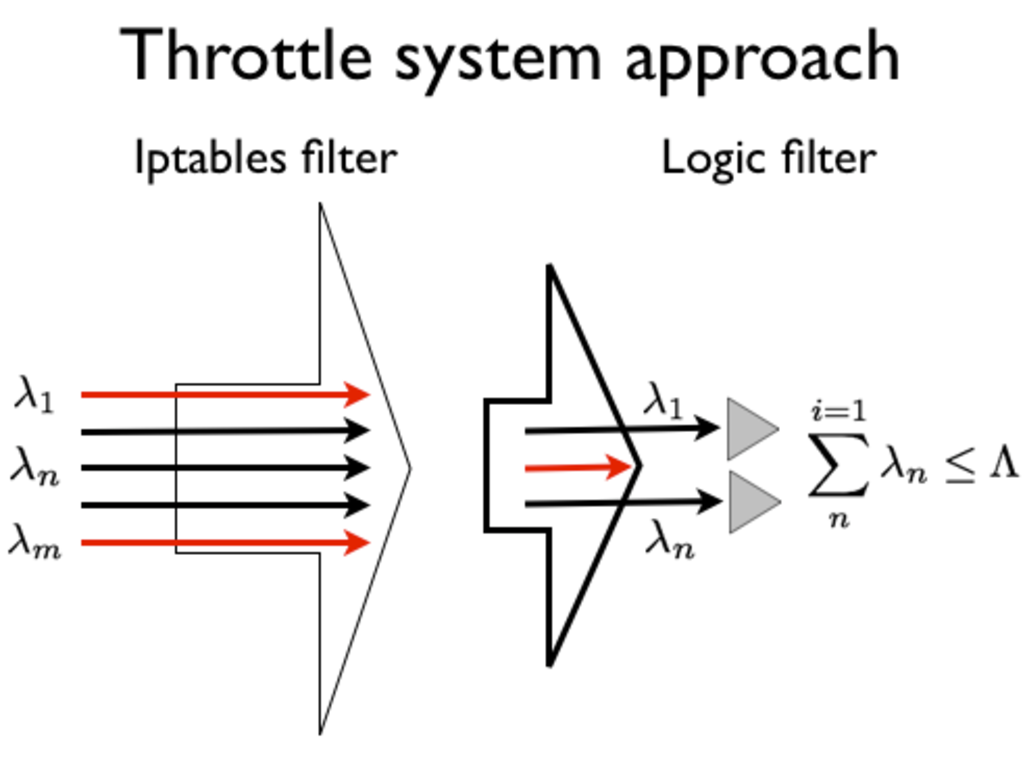
\includegraphics[width=0.6\textwidth]{img/throttle_system.pdf}
\caption{Stages at Throttle system}
\end{center}
\end{figure}

 
 
 Iptables commands\footnote{\url{http://www.debian-administration.org/articles/187}} holding the theory are:
\begin{verbatim}
iptables -I INPUT -p tcp --dport 8000 -i eth0 -m state --state NEW -m recent \
  --set

iptables -I INPUT -p tcp --dport 8000 -i eth0 -m state --state NEW -m recent \
  --update --seconds 6 --hitcount 40 -j DROP
\end{verbatim} 
 
 A simple implementation of Soft layer could be:
 \begin{itemize}
\item Structure to manage several tokens:
\begin{verbatim}
# Tokens control
tokens = {}
tokens['d41d8cd98f00'] = {}
tokens['d41d8cd98f00']['hits'] = 0
tokens['d41d8cd98f00']['timestamp'] = time.time()

tokens['204e9800998e'] = {}
tokens['204e9800998e']['hits'] = 0
tokens['204e9800998e']['timestamp'] = time.time()

......
\end{verbatim} 


\item Time control to throttle requests over a token (inthis case 3 request per second are allowed):
 \begin{verbatim}
# Token control
valid_request = True

# Get token param
token = self.get_argument("token")

if token not in self.tokens:
    result = {'error': 'token is not valid'}
    valid_request = False
else:
    if time.time() - self.tokens[token]['timestamp'] < 1:
        self.tokens[token]['hits'] += 1
        if self.tokens[token]['hits'] > 3:
            result = {'error': 'rate limited'}
            valid_request = False
    else:
        self.tokens[token]['timestamp'] = time.time()
        self.tokens[token]['hits'] = 0

if valid_request:
# Service processing start
\end{verbatim} 
 \end{itemize}
 
 






 \newpage
 \section{Simulation to find paramaters (\lambda, \mu, \rho, ...) }
By means of the software developed at Paradigma Labs\footnote{\url{https://github.com/rmaestre/mmck-CTMarkovChain}}, we can see more parameters like tail configuration, waiting times, etc ...
\\
Here, we now that we can process $400$ words in 0.5 secs plus 1.0 of time wasted in the network, so, in one atomic request service time will be $1.5$. We are establish the Iptables filter in 3 users and each user is allow to perform 3 request persecond. Our server is going to run $4$ paralell threads, therefore, we have a $\lambda = 3 * 3 = 9 / \text{secs}.$, $\mu = 1.5 / \text{secs}.$, $c=4$ and $k = 100$. 
\\
\\
Simulation shows that we are going to {\bf need $7$ server threads running} to support the load ($\rho < 1$)

\begin{verbatim}

Roberto-Maestres-MacBook-Pro:mmck-CTMarkovChain rmaestre$ python simulate.py 

+ MODEL PARAMETERS
	Lambda: 9.0000
	Mu: 1.5000
	c: 7.0000
	K: 100.0000
	Stability: True (rho = 0.8571)

+ TAIL
	Average number of clients (l) = 9.6830
	Average length (lq) = 3.6830
	Average waiting time for a client into the tail (w) = 1.0759

+ SYSTEM
	Average waiting time into the system (wq) = 0.4092

+ PROBABILITY DISTRIBUTION
	P_0 = 0.0015787817
	P_1 = 0.009472690047149
	P_2 = 0.028418070141446
	P_3 = 0.056836140282893
	P_4 = 0.085254210424339
	P_5 = 0.102305052509207
	P_6 = 0.102305052509207
	P_7 = 0.087690045007892
	P_8 = 0.075162895721050
	P_9 = 0.064425339189471
	P_10 = ..... 
	..... 
	P_100 = 0.000000052107334
	[Total Probability: 1.0]

Elapsed time: 0.00043821
\end{verbatim}




 


\newpage
\section{Results}
If we have a $\lambda = 2.78 sec$ ,and we have a Service Time $\mu = 1.5 sec.$ we can trace the $\rho$ parameter:
\begin{figure}[htb]
\begin{center}
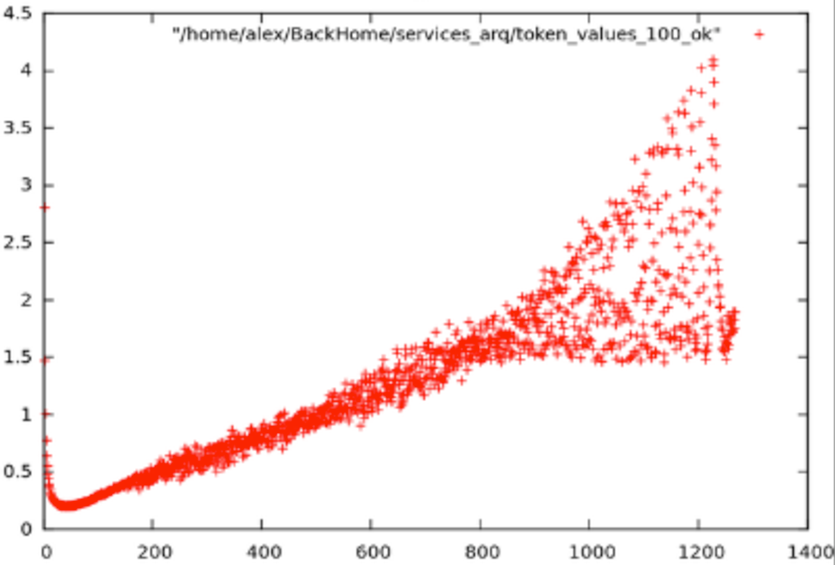
\includegraphics[width=0.6\textwidth]{img/time_service.pdf}
\caption{Service times in several set of configurations}
\end{center}
\end{figure}
Now, we can study the behavior of the tail and the system for several set of configurations.


\begin{figure}[htb]
\begin{center}
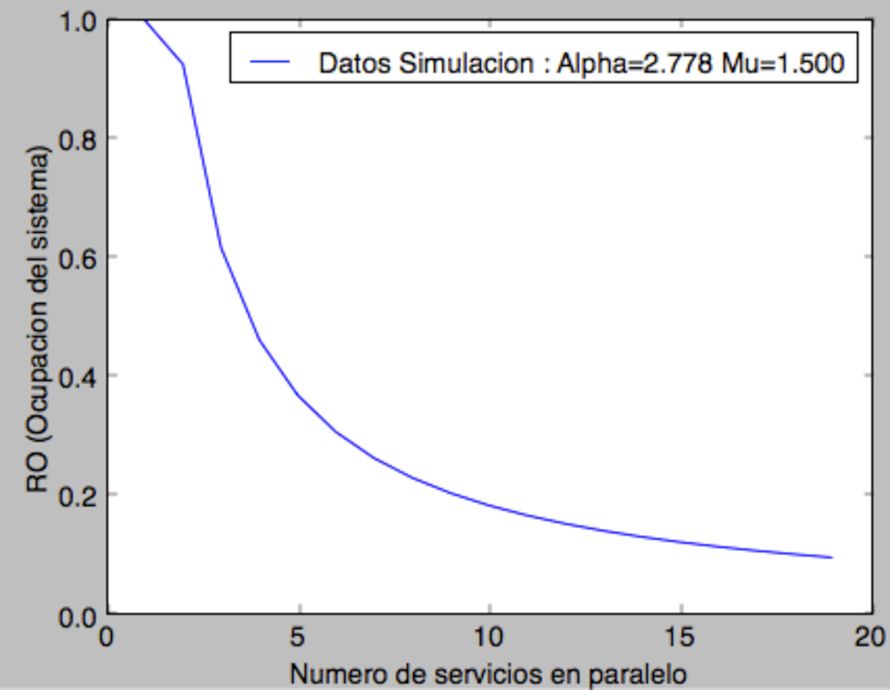
\includegraphics[width=0.6\textwidth]{img/simulation_1.pdf}
\caption{Service times in several set of configurations}
\end{center}
\end{figure}


As we can see in the next picture, this parameters woorking nice with the simulated configuration.
\newpage
\begin{figure}[htb]
\begin{center}
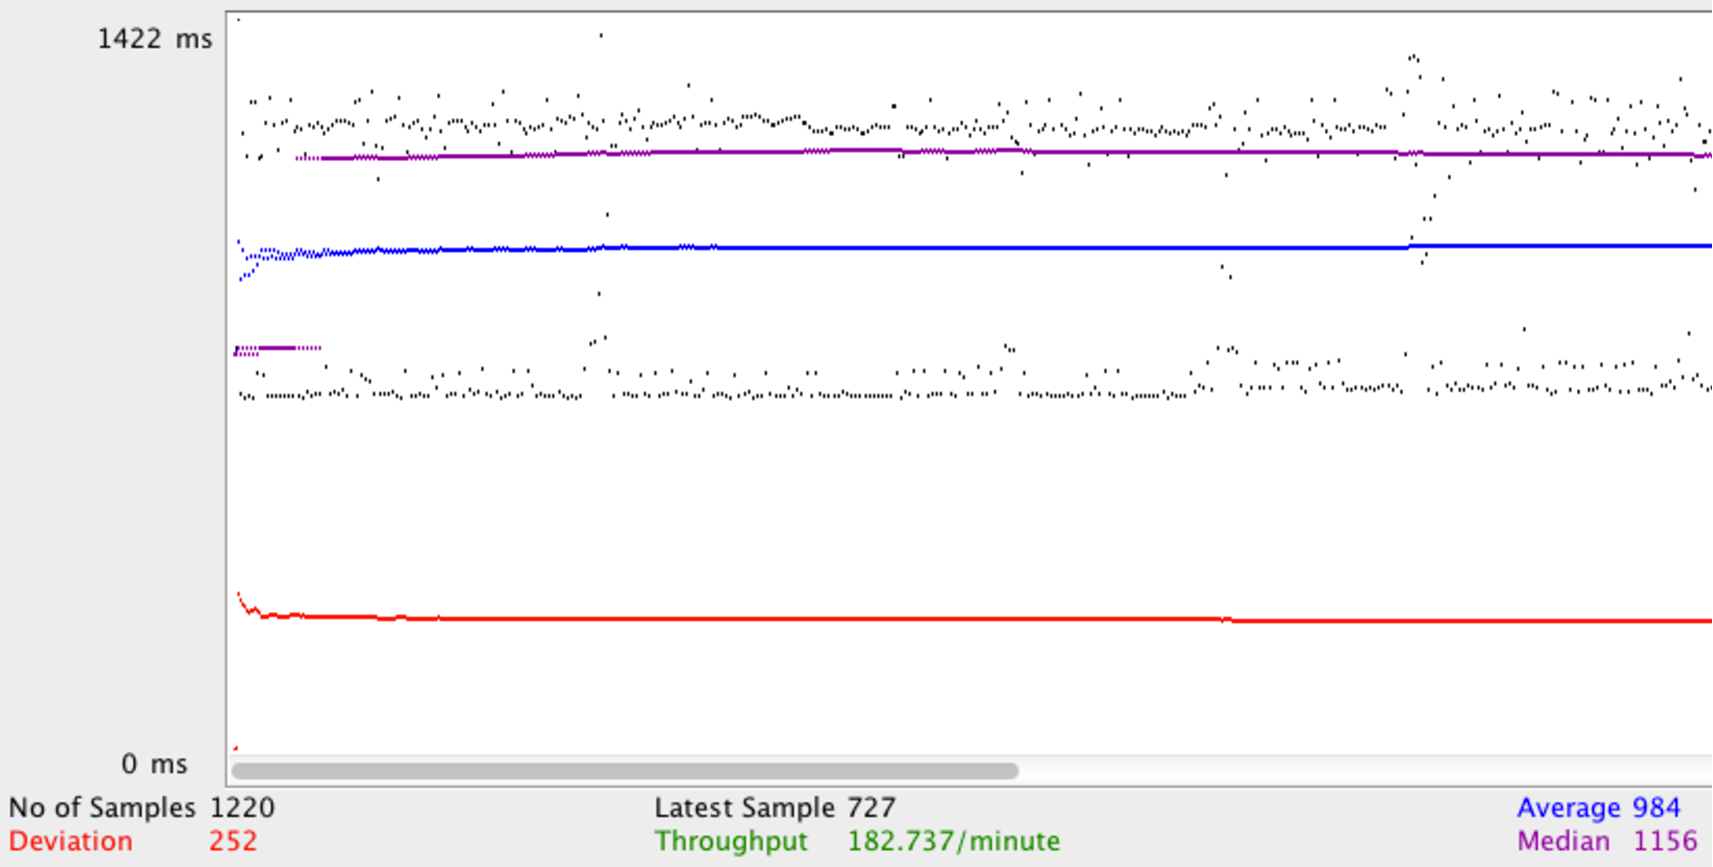
\includegraphics[width=0.7\textwidth]{img/apache_jmeter.pdf}
\caption{Testing real service}
\end{center}
\end{figure}

\begin{figure}[htb]
\begin{center}
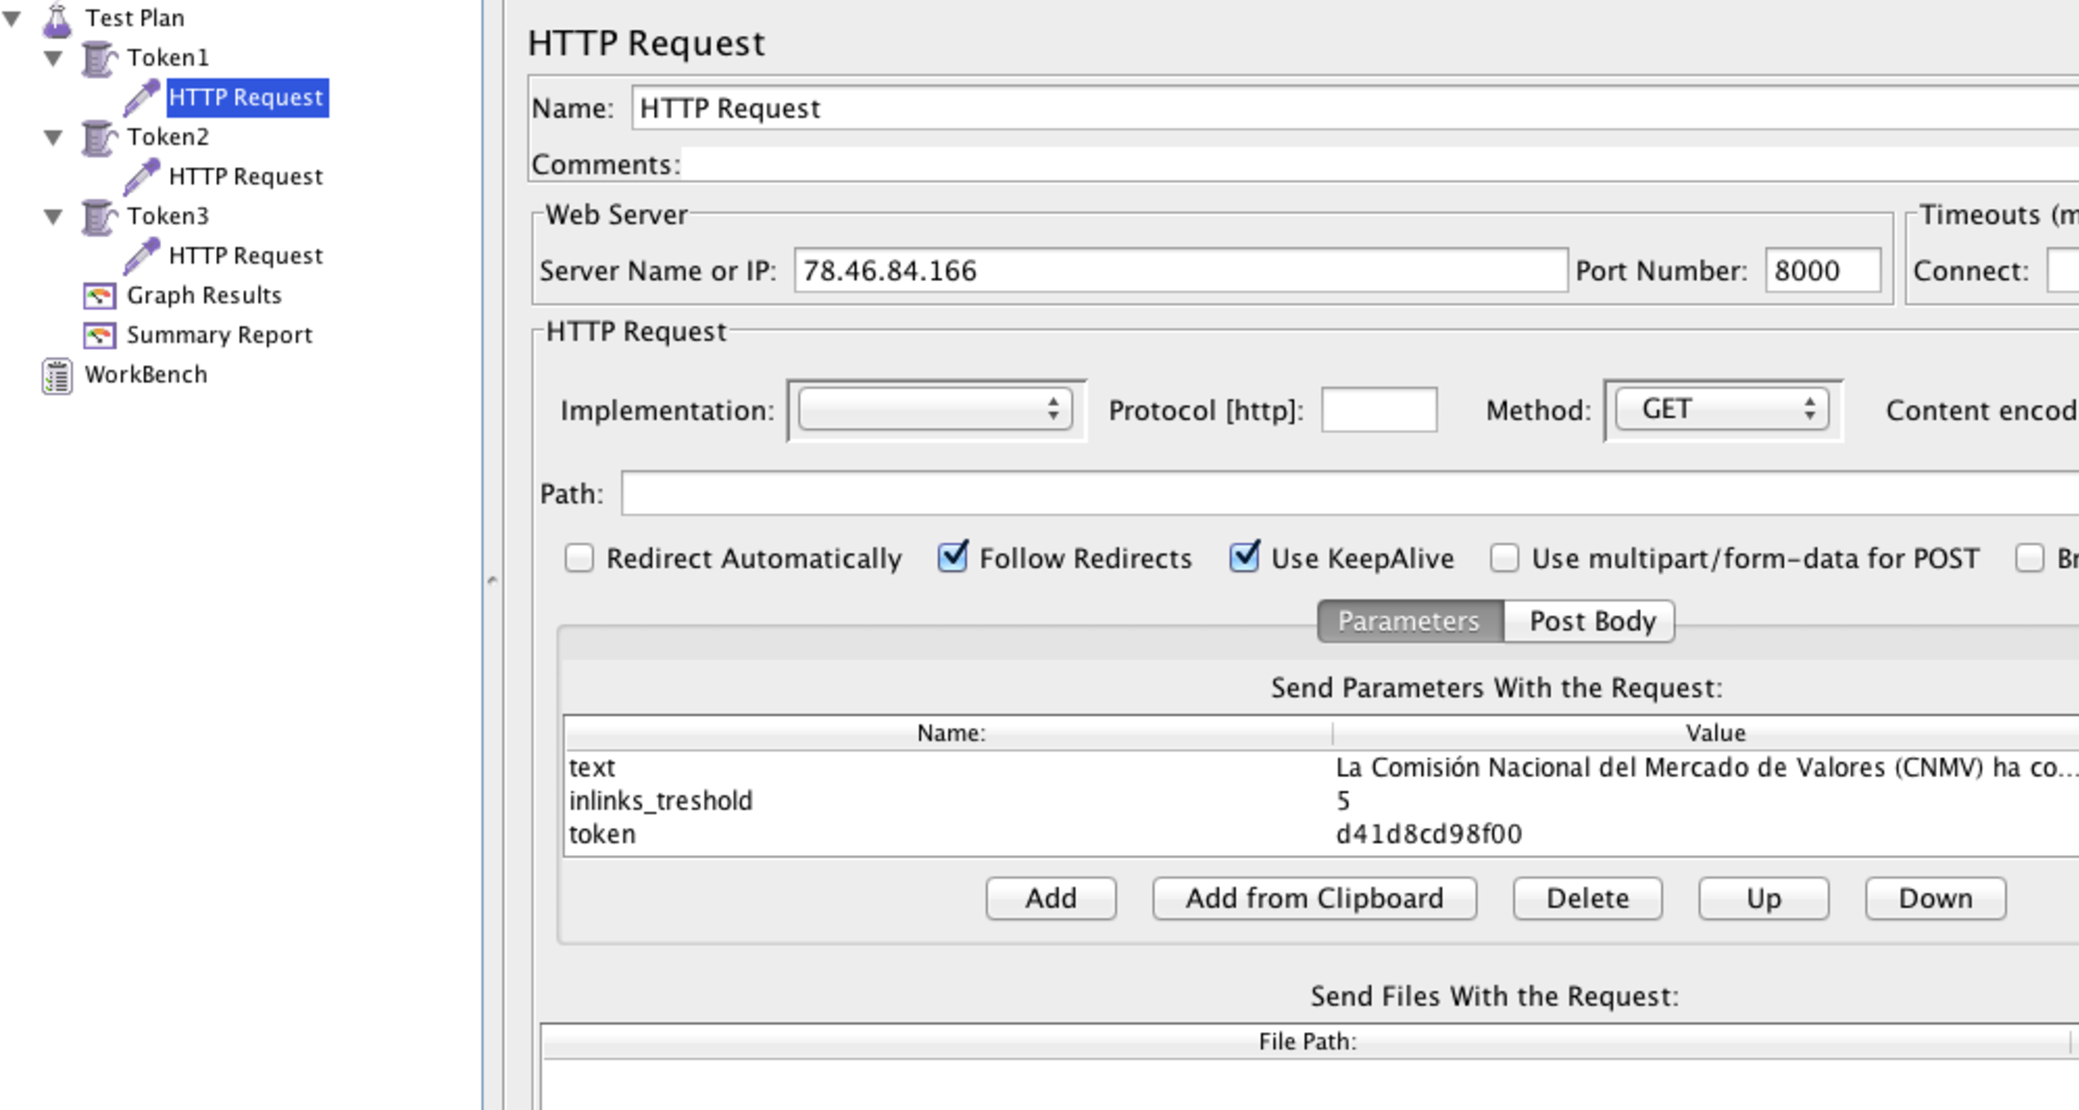
\includegraphics[width=0.6\textwidth]{img/jmeter_conf.pdf}
\caption{Apache JMeter configuration}
\end{center}
\end{figure}

\newpage
\section{Conclusions}
\begin{itemize}
\item Using wikipedia categories and articles, we are able to detect a huge range of Entities.
\item Wikipedia is always updated in real time, therefore we have a updated NER.
\item We can use Gunicorn to manage serveral service threads.
\item We are implemented a Throttle service to restrict the maximun number of request per second. Also is provided the way to restrict the general service by means of $iptables$.
\item It is important simulate our service like a tail through Continuos-time Markov Chain in order to find important variables like $\lambda, \mu, \rho, L, L_q, W, W_q$.
\end{itemize}


\newpage
\bibliographystyle{plainnat}
\bibliography{biblio}

\end{document}
